% doc/impl/impl.tex
% Implementierungstechnische Details, Programmbeschreibung 
%
% Ausarbeitung zur Diplomarbeit Nr. 2035 - "Erzeugung und Evaluierung 
% von Oktalbaumstrukturen als Schnittstelle zu CAD-Programmen"
%   
% Autor: Stefan Mahler 2002
%   Universitaet Stuttgart, SgS
% Betreuer: Ralf Mundani

\chapter{Implementierung}
\label{impl}
Dieses Kapitel besch"aftigt sich mit der innerhalb dieser Arbeit erzeugten 
Implementierung. Programmaufbau und Programmoptionen werden im Abschnitt 
\ref{umsetzung} beschrieben. Ergebnisse bez"uglich Zeit- und 
Speicheraufwand bei der Oktalbaumgenerierung mit dieser Implementierung sind 
im Abschnitt \ref{leistungstest} zu lesen.

\section{Umsetzung}
\label{umsetzung}
Zun"achst soll auf einige implementierungstechnischen Besonderheiten 
eingegangen werden. Anschlie"send erfolgt im Abschnitt \ref{prg_descr} 
eine Beschreibung der erstellten Implementierung. 

\subsection{Einige implementierungstechnische Details} 
Zur Implementierung wurde die Programmiersprache C++ verwendet. 
Einschl"agige C++-Compiler sind f"ur alle g"angigen Betriebsysteme, 
insbesondere f"ur alle Unix-Derivate wie Linux und alle Windows-Varianten 
verf"ugbar. Der Quellcode kann somit auf unterschiedlichen Plattformen 
"ubersetzt werden. 

In C++ k"onnen Programme im objekt-orientierten Programmierstil erstellt 
werden. In der hier erzeugten Implementierung wurde 
unter anderem von den Mitteln des Exception Handling, des Polymorphismus und 
des Overloading und der Unterst"utzung von Assertions Gebrauch gemacht. 
C++ l"asst die Erzeugung von hochperformantem Code  zu. (In dieser Arbeit 
wurde der \texttt{g++}-Compiler mit der Option \texttt{-O3} verwendet.)

Wegen ihrer hohen Popularit"at existieren eine Vielzahl von 
Ver"offentlichungen zu C++. Neben Werken, die eine "Ubersicht "uber die 
Programmiersprache geben (z.B. \cite{prgspr_cpp}), gibt es Abhandlungen 
zu speziellen Merkmalen von C++, wie die 
STL\footnote{Standard Template Library: Bibliothek, die grundlegende 
Datenstukturen wie Listen, beliebig lange Felder und Zeichenketten (Strings) 
oder Str"ome (Streams) enth"alt.} (z.B. \cite{stl}) oder algorithmische 
Umsetzungen in C++(\cite{algo_cpp}), die auch in dieser Arbeit verwendet 
wurden. Zus"atzlich finden sich Bibliotheken f"ur konkrete Aufgabenstellungen, 
die sich einfach verwenden lassen. Ein Beispiel hierf"ur ist 
\emph{dime}, eine Bibliothek, 
die zum Einlesen der Oberfl"achenmodelle 
im DXF-Format (vgl. Abschnitt \ref{dxf_bibliotheken}) benutzt wird.

\label{option_switch}
Eine Besonderheit von C++ ist die Verwendbarkeit von sogenannten 
Pr"aprozessormakros. Sie wurden z.B. f"ur \emph{Optionsschalter} eingesetzt. 
Soll das Programm mit eingeschalteten Option 'XYZ' compiliert werden, 
so muss in \texttt{global.h} die Zeile 
\begin{alltt}
\#define XYZ
\end{alltt}
stehen. Zum Ausschalten der Option 'XYZ' muss diese vor erneuter Compilierung 
durch \texttt{//} auskommentiert werden. 
In der Datei \texttt{global.h} steht also 
\begin{alltt}
//#define XYZ
\end{alltt}
anstatt obiger Zeile. Zum Wiedereinschalten wird \texttt{//} wieder entfernt. 
Im ausf"uhrbaren Programm sind somit immer nur Methoden zu einer 
Optionsschalterstellung (ein \emph{oder} aus) enthalten. Optionen, die 
sich von Programmlauf zu Programmlauf "andern k"onnen, werden als 
Programmparameter beim Programmstart "ubergeben. "Uber alle Optionsschalter 
und Programmparameter gibt Abschnitt \ref{prg_descr} Auskunft.

Zum besseren Verst"andnis des Quellcodes wurde eine Klassenreferenz mit Hilfe 
von \emph{doxygen} (\cite{doxygen}) generiert.

Wegen ihrer herausragenden Bedeutung soll hier die implementierte 
Zeigerstruktur des Oktalbaums vorgestellt werden 
(vgl. Abbildung \ref{oct_struct}): 

\diabeg
\begin{alltt}
\struct{Node}
\typedef{Node* \_octree}

\struct{Node \{
  \struct{\_octree parts}
  Color flag;
\}} 
\end{alltt}
\caption{Implementierte Zeigerstruktur des Oktalbaums}\label{oct_struct}
\diaend

Ein Knoten besteht aus einer Referenz auf seine S"ohne \texttt{parts} und 
einem Status-Attribut \texttt{flag}. F"ur Bl"atter ist 
\texttt{parts}~$=$~\texttt{NULL} und \texttt{flag} enth"alt die Knotenfarbe. 
F"ur innere Knoten referenziert \texttt{parts} die acht Sohnknoten, 
\texttt{flag} ist undefiniert. 
\texttt{parts} wird f"ur innere Knoten dynamisch als Feld erzeugt. 
Durch das gemeinsame Abspeichern aller S"ohne hintereinander und die Nutzung 
nur einer Referenz 
\begin{itemize}
\item ist gew"ahrleistet, dass ein Knoten entweder genau acht oder gar kein 
    Sohn hat. Der erzeugte Baum ist somit immer ein Oktalbaum im Sinne der 
    Definition. 
\item wird weniger Speicherplatz ben"otigt, da nur einer anstatt acht Zeiger  
    f"ur die acht S"ohne eines inneren Knotens ben"otigt wird.
\end{itemize}
Diese Datenstruktur wurde bereits in anderen Implementierungen als 
Oktalbaumstruktur von der Abteilung Simulation gro"ser Systeme eingesetzt und 
hat sich dort bew"ahrt. 
Des Weiteren ist gew"ahrleistet, dass die Wurzel eines Oktalbaums immer 
referenzierbar ist, auch wenn der Oktalbaum kein Geometrie-Modell enth"alt. 

F"ur jeden Knoten des Oktalbaums werden in den verwendeten Testumgebungen 
64 Bytes Speicher alloziert.

\subsection{Programmbeschreibung} 
\label{prg_descr}
Mit \textbf{cad2octree} l"asst sich zu einem gegebenen Oberfl"achen-Modell 
ein Oktalbaum generieren, der das gleiche Modell repr"asentiert.

\begin{description}
\item[Anforderungen an das gegebene Oberfl"achenmodell]\label{%
    oberflmodel_anf}~\\
    Das Oberfl"achenmodell stellt einen Rigid Body dar. Als Format wird DXF 
    verwendet. Zur Modellierung von glatten Oberfl"achen wurde die ENTITY 
    \texttt{3DFACE}, f"ur Spline-Oberfl"achen die ENTITY \texttt{POLYLINE} 
    benutzt. (Es werden nur \texttt{POLYLINE}-Entities vom Oberfl"achentyp 
    \emph{Cubic B-spline surface} (Group code 75), dem Typ 
    \emph{polygon mesh} und dem Flag \emph{Spline-fit, 3D polygon mesh} 
    (Groupcode 70) ausgewertet, vgl. Abschnitt \ref{import} und 
    \cite[S. 62, 97]{dxf_ref}.) 
\item[Erzeugter Oktalbaum]~\\ 
    Der generierte Oktalbaum wird in Pr"aorder-Traversierung als Bin"arstrom 
    geschrieben, vgl. Abschnitt \ref{export_pot}.
\item[Programmparameter]~\\ 
    \emph{cad2octree} wird durch: 

    \texttt{cad2octree [-q] [-d <depth>] <input> [-o <output>]}

    aufgerufen. Dabei ist: 

    \begin{tabularx}{\linewidth}{p{1.7cm}X}
	 -q       & die Option, die das Aufpalten von Vierecken in 
		    $2$ Dreiecke erzwingt. 
    \end{tabularx}
    \begin{tabularx}{\linewidth}{p{1.7cm}X}
	 <depth>  & die maximale Baumtiefe 
    \end{tabularx}
    \begin{tabularx}{\linewidth}{p{1.7cm}X}
	 <input>  & der Name der Eingabedatei. Das ist die DXF-Datei, die das
		    Oberfl"achenmodell ent"alt. Sie muss die Erweiterung 
		    \texttt{dxf} oder \texttt{dxb} besitzen. 
    \end{tabularx}
    \begin{tabularx}{\linewidth}{p{1.7cm}X}
         <output> & der Name der Ausgabedatei f"ur den Oktalbaum als 
		    Bin"arstrom in Pr"aordertraversierung. Der Dateiname muss 
		    die Endung \texttt{pot} haben. Wird nur die Eingabedatei, 
		    aber keine Ausgabedatei angegeben, wird der Oktalbaum zur 
		    Eingabedatei \emph{xyz}\texttt{.dxf} in die Ausgabedatei 
		    \emph{xyz}\texttt{.pot} geschrieben. 
    \end{tabularx}
\item[Optionsschalter]~\\ 
    Mit \emph{cad2octree} ist es prinzipiell m"oglich, aus unterschiedlichen 
    Verfahren einen Algorithmus zur Oktalbaumgenerierung auszuw"ahlen. 
    Die Optionsschalter m"ussen \emph{vor} dem Compilieren von cad2octree 
    festgelegt werden (vgl. Abschnitt \ref{option_switch}). 
    Einige Optionsschalter sind nur in Verbindung mit anderen wirksam. 
    So ist z.B. \switch{ALGORITHM\_CHECK\_DET} nur wirksam, 
    falls \switch{ALGORITHM\_ISIN} eingeschaltet ist und 
    \switch{ALGORITHM\_ISIN} hat nur eine Wirkung, wenn \switch{CLASSIC\_MODE} 
    ausgeschaltet ist. 
    Diese Abh"angigkeiten werden aus der Zuordnung der Optionsschalter 
    in der folgenden Beschreibung ersichtlich. \textbf{\emph{ein}} steht 
    f"ur einen eingeschalteten, \textbf{\emph{aus}} f"ur einen ausgeschalteten 
    Optionsschalter. Fehlt die Angabe \textbf{\emph{ein}} bzw. 
    \textbf{\emph{aus}}, ist immer der eingeschaltete Optionsschalter gemeint. 

    \newcommand*\option[1]{\textbf{\switch{#1}}}
    \newcommand*\opton{\textbf{\emph{ein}:}~}
    \newcommand*\optoff{\textbf{\emph{aus}:}~}
    \newcommand*\see{$\leadsto$ }

    \option{CLASSIC\_MODE}
    \begin{itemize}
    \item\optoff Nutze ein Alternativverfahren.
    
	\option{FILL\_SOLIDS}
	\begin{itemize}
	\item\optoff Es wird ausschlie"slich die K"orperoberfl"ache erzeugt. 
	\item\opton Nach der Generierung der K"orperoberfl"ache wird ein 
	    F"ullalgorithmus gestartet und danach kompaktiert. 
	    
	    \option{MARK\_BORDER:} Der Rand des F"ullgebiets wird beim 
		Erreichen der Rekursionstiefe \const{MAX\_RECURSIVE\_DEEP} 
		innerhalb der Funktion \func{fill}{} mit der 
		entsprechenden Randfarbe markiert und der F"ullalgorithmus 
		abgebrochen.
	    
	    \option{LIMITED\_STACK:} Beim Erreichen der Rekursionstiefe 
		\const{MAX\_RECURSIVE\_DEEP} innerhalb der Funktion 
		\func{fill}{} wird der F"ull\-algo\-rith\-mus abgebrochen und 
		auf einem zuvor gemerkten Punkt wieder aufgesetzt.
	    
	    \hide{\option{USE\_QUEUE:} Anstatt des rekursiven Aufrufs von 
		\func{fill}{} wird eine \emph{Queue} zum Merken der 
		Knoten der F"ullfront verwendet.} 
	\end{itemize}

	\option{ALGORITHM\_ISIN}
	\begin{itemize}
	\item\optoff Das Scan-Line-Verfahren wird verwendet.
	    
	    \option{COMB\_SCAN\_LINE}
	    \begin{itemize}
	    \item\optoff Als Nachbarpunkte werden nur die Nachbarn entlang 
		der Achsrichtungen angesehen. 
	    \item\opton Als Nachbarpunkte k"onnen auch die Nachbarn entlang 
		der Diagonalrichtungen angesehen werden.  
	    \end{itemize}
	\item\opton Es wird ein hybrides Verfahren eingesetzt, d.h. der 
	    K"orperrand wird "uber den rekursiven Abstieg mit Hilfe 
	    des Teststrahlverfahrens auf den Oberfl"achenpolygonen 
	    generiert.
	
	    \option{ALGORITHM\_CHECK\_DET}
	    \begin{itemize}
	    \item\optoff Ob ein Punkt in der Polygonebene liegt, wird "uber 
		seinen Abstand zum Fu"spunkt bestimmt.
	    \item\opton Ob ein Punkt in der Polygonebene liegt, wird 
		mit Hilfe des Determinantenverfahrens bestimmt.
	    \end{itemize}
	\end{itemize}
    \item\opton Nutze das klassisches Verfahren. Der Oktalbaum wird mit Hilfe 
	des rekursiven Abstiegs erzeugt.
	\hide{\paragraph{CM\_PART} Es werden nur die Polygone des 
	    CAD-Modells betrachtet die duch den Teststrahl ausgehend von 
	    der Vaterknoten-Zelle geschnitten wurden.}
    \end{itemize}
    
    \option{NDEBUG} 
    \begin{itemize}
    \item\optoff Die "Uberpr"ufungen durch Assertions sind eingeschaltet. Dies 
	ist w"ahrend dem Entwicklungsstadium des Programms hilfreich, da 
	dadurch m"ogliche Fehler in der Implementierung besser eingegrenzt
	werden k"onnen. 
	So wird z.B. vor der Bestimmung der Farbe eines Knotens durch 
	\func{getColor}{} "uberpr"uft, ob der Knoten ein Blatt innerhalb 
	des Oktalbaums ist. 
    \item\opton Es werden keine zus"atzlichen "Uberpr"ufungen durch 
	\emph{Assertions} durchgef"uhrt, 
	was die Ausf"uhrgeschwindigkeit des Programms erh"oht. 
    \end{itemize}
\item[Unterst"utzte Plattformen]~\\ 
    Das Programmpaket ist in C++ nach dem ANSI C++ - Standard entwickelt 
    worden. Es sollte somit auch mit einem beliebigen ANSI C++ - konformen 
    Compiler "ubersetzbar und ausf"uhrbar sein. Zum "Ubersetzen bzw. zum 
    Ausf"uhren von cad2octree wird dime ben"otigt. 
    Wird die Ausf"uhrung abgebrochen, da dime nicht gefunden werden kann, 
    obwohl es installiert ist, kann evtl. das Hinzu"ugen des 
    Verzeichnisses, indem sich die compilierte dime-Bibliothek 
    \texttt{libdime.la} befindet, zur Umgebungsvariable 
    \texttt{LD\_LIBRARY\_PATH} helfen. 
\item[Compilieren der Sourcen]~\\
    Als erstes muss \emph{dime} installiert werden (eine 
    Installationsanleitung ist im dime-Programmpaket enthalten). 
    Zum Compilieren k"onnen die \texttt{Makefile}s verwendet werden, falls 
    \emph{gmake Version 3.79} oder kombatibel installiert ist. 
    Vor dem Aufruf von \texttt{make} im \texttt{src}-Verzeichnis zum 
    Compilieren der Sourcen m"ussen die Pfadangaben in \texttt{Makefile.incl} 
    (im Projekthauptverzeichnis) angepasst werden:
    \begin{itemize}
    \item \texttt{INCLUDES} muss das dime-Include-Verzeichnis enthalten. 
    \item \texttt{LDFLAGS} muss das Verzeichnis enthalten, indem die 
	compilierte dime-Bibliothek steht. 
    \item Eventuell m"ussen noch die Angaben bei \texttt{CC}, \texttt{LD} 
	und \texttt{AR} (entsprechend auch bei \texttt{CCFLAGS}, 
	\texttt{LDFLAGS} und \texttt{ARFLAGS}) angepasst werden, falls ein 
	anderer Compiler als \texttt{g++} verwendet wird, bzw. \texttt{ld} 
	nicht als Linker oder \texttt{ar} zur Codeerzeugung nicht zur 
	Verf"ugung stehen. 
    \end{itemize} 
    Alternativ zur Nutzung von \texttt{make} kann cad2octree auch direkt 
    unter Angabe aller Programmbibliotheken (einschlie"slich dime) "ubersetzt 
    werden. 
\item[Verwendete Bibliotheken Dritter]~\\
    cad2octree verwendet die DXF-Bibliothek \textbf{dime} \cite{dime}. 
    Es ist die GPL Version 2 zu beachten\footnote{Zu finden unter: 
    \url{http://www.gnu.org/licenses/gpl.txt}, \\ Deutsche "Ubersetzung: 
    \url{http://www.gnu.de/gpl-ger.html}}. 
\end{description}

%%%%%%%%%%%%%%%%%%%%%%%%%%

% doc/impl/test.tex
% Leistungstest (verwendete Modelle, Testumgebung, Testresultate)
%
% Ausarbeitung zur Diplomarbeit Nr. 2035 - "Erzeugung und Evaluierung 
% von Oktalbaumstrukturen als Schnittstelle zu CAD-Programmen"
%   
% Autor: Stefan Mahler 2002
%   Universitaet Stuttgart, SgS
% Betreuer: Ralf Mundani

\section{Leistungstest}
\label{leistungstest}
Wie bereits im letzten Abschnitt erl"autert wurde, sind in \emph{cad2octree} 
verschiedene Verfahren zur Oktalbaumgenerierung implementiert worden. 
Diese Verfahren wurden mit Hilfe von unterschiedlichen Modellen (vgl. 
Abschnitt \ref{models}) auf den im Abschnitt \ref{testenv} beschriebenen 
Systemen ausgef"uhrt. Die Ergebnisse (insbesondere Laufzeit- und 
Speicherbedarf-Vergleiche) sind in Abschnitt \ref{test_results} aufgelistet. 

\subsection{Verwendete Modelle}
\label{models}
Die verwendeten Oberfl"achenmodelle lassen sich in zwei Gruppen unterteilen. 
W"ahrend die Modelle der ersten Gruppe nur glatte Oberfl"achen besitzen, 
wurden bei den Modellen der zweiten Gruppe auch (oder ausschlie"slich) 
kubische B-Spline-Fl"achen eingesetzt. 

Zur Erzeugung der Oberfl"achenmodelle im DXF-Format wurde ausschlie"slich 
Maya Unlimited 4.0 von Alias|Wavefront 
eingesetzt. 

Die (Datei-)Namen der Modelle werden ohne die Erweiterung \emph{.dxf} 
angegeben. Abk"urzend wird f"ur \emph{2\_kugeln\_nurbs\_u\_poly.dxf} nur 
\emph{2\_kugeln} geschrieben. 

\subsubsection{Modelle mit polygonaler Oberfl"ache}
\label{models_plane}
In Tabelle \ref{tbl_models_plane} sind die verwendeten Modelle mit 
ausschlie"slich glatten Oberfl"achen aufgelistet.

\tabbeg
\newcounter{piccount}
\newcommand\picref{
    \stepcounter{piccount}\ref{abb_models_plane} \alph{piccount})}
\newcommand\myitem[7]{\hline \emph{#1} & {\hfill #2} & {\hfill #3} & 
    {\hfill #4} & {\hfill #5} & {\hfill #6} & {\hfill #7}}
\begin{tabularx}{\linewidth}{|l|c|X|X|c|X|c|}
\hline
\bf\emph{Modell} & \bf bungalow & \bf {\hfil gear} & \bf {\hfil gear2} 
    & \bf kugel\_poly & \bf {\hfil ship} & \bf wuerfel \\
\myitem{\# Vertices}{1 200}{1 440}{9 940}{1 560}{3 712}{24}\\
\myitem{\# Dreiecke}{  200}{    0}{  100}{   40}{    0}{ 0}\\
\myitem{\# Vierecke}{  150}{  360}{2 410}{  360}{  928}{ 6}\\
\myitem{Dateigr"o"se [kB]}{104}{114}{738}{104}{270}{2}\\
\myitem{Abbildung}{\picref}{\picref}{\picref}{\picref}{\picref}{\picref}\\
\hline
\end{tabularx}
\tabend{tbl_models_plane}{Modelle mit polygonaler Oberfl"ache}

\begin{figure}
\begin{center}
\setcounter{piccount}{0}
\newcommand*\picname[1]{\stepcounter{piccount}\alph{piccount}) \emph{#1}}
\newcommand\mypics[4]{\extpic{#1}  & & \extpic{#3} \\ 
		      \picname{#2} & & \picname{#4} \\}
\begin{tabular}{cp{0.5cm}c}
    \mypics{bungalow}{bungalow}{gear}{gear} \\ 
    \mypics{gear2}{gear2}{kugel_poly}{kugel\_poly} \\
    \mypics{ship}{ship}{wuerfel}{wuerfel}
\end{tabular}
\caption{Modelle mit polygonaler Oberfl"ache}
\label{abb_models_plane}
\end{center}
\end{figure}

\begin{description}
\item[bungalow] Modell eines kleinen Gartenshauses. Die einzelnen Bauteile 
    wie Decke, Boden, W"ande, St"utzpfeiler und Fensterrahmen wurden als 
    separate Teile modelliert. 
\item[gear] Modell eines einzelnen Zahnrads. Das Zahnrad enth"alt in der Mitte 
    eine Bohrung. 
\item[gear2] In der Mitte des Modells befindet sich ein Sonnenritzel  
    (ohne Bohrung), um welches sich innerhalb des Planetentr"agers 
    $4$ Planeten um das Sonnenritzel drehen. Unter den getesteten Modellen 
    mit rein polygonaler Oberfl"ache ist es das Komplexeste.  
\item[kugel\_poly]\label{model_kugel_poly} 
    Modell einer durch polygonale Oberfl"achenst"ucke approximierten Kugel. 
\item[ship] 
    Modell eines Raumschiffs. Es enth"alt Einbuchtungen, ist also nicht 
    vollst"andig konvex. 
\item[wuerfel]
    Achsparalleler W"urfel. Das einfachste getestete Modell. 
\end{description}

\subsubsection{Modelle mit Spline-Oberfl"ache}
Tabelle \ref{tbl_models_spline} gibt einen "Uberblick "uber die verwendeten 
Modelle, die B-Spline-Oberfl"achen enthalten. 

\tabbeg
\setcounter{piccount}{0}
\newcommand\picref{
    \stepcounter{piccount}\ref{abb_models_spline} \alph{piccount})}
\newcommand\myitem[5]{\hline %
    \emph{#1} & {\hfill #2} & {\hfill #3} & {\hfill #4} & {\hfill #5}}
\begin{tabularx}{\linewidth}{|l|X|X|X|X|}
\hline
\bf\emph{Modell} & \bf {\hfil 2\_kugeln} & \bf {\hfil gelenk} & 
    \bf {\hfil kugel\_nurbs} & \bf {\hfil sgs\_logo}\\
\myitem{\# Splinefl"achen}{    1}{   13}{  1}{  114}\\
\myitem{\# Kontrollpunkte}{  176}{2 273}{176}{5 168}\\
\myitem{\# Vertices      }{1 736}{2 273}{176}{5 168}\\
\myitem{\# Dreiecke      }{   40}{    -}{  -}{    -}\\
\myitem{\# Vierecke      }{  360}{    -}{  -}{    -}\\
\myitem{Dateigr"o"se [kB]}{131}{445}{27}{826}\\
\myitem{Abbildung}{\picref}{\picref}{\picref}{\picref}\\
\hline
\end{tabularx}
\tabend{tbl_models_spline}{Modelle mit Spline-Oberfl"ache}

\begin{figure}[ht]
\begin{center}
\setcounter{piccount}{0}
\newcommand*\picname[1]{\stepcounter{piccount}\alph{piccount}) \emph{#1}}
\newcommand\mypics[4]{\extpic{#1}& &\extpic{#3}\\ 
		      \picname{#2} & & \picname{#4} \\}
\begin{tabular}{cp{0.5cm}c}
    \mypics{2_kugeln}{2\_kugeln}{gelenk}{gelenk} \\ 
    \mypics{kugel_nurbs}{kugel\_nurbs}{sgs_logo}{sgs\_logo}
\end{tabular}
\caption{Modelle mit Spline-Oberfl"ache}
\label{abb_models_spline}
\end{center}
\end{figure}

\begin{description}
\item[2\_kugeln] Modell zweier nebeneinanderliedenen Kugeln. Die eine 
    Kugeloberfl"ache ist durch Polygone approximiert, die andere Kugel 
    durch eine Spline-Fl"ache modelliert. 
\item[gelenk] Das Modell besteht aus sieben Segmenten. Das Mittelsegment 
    ist eine Kugel. In jeder Achsrichtung schlie"sen sich beidseitig 
    Zylinder (Tuben) an. Alle Segment\-oberfl"achen sind abgeschlossen und 
    durch Spline-Fl"achen modelliert. 
\item[kugel\_nurbs] Eine Kugel, die durch eine Spline-Fl"ache modelliert ist. 
\item[sgs\_logo] Das Modell zeigt einen d"unnen Torus, der sich in einem 
    Oktalbaumgitter (als Rohre) befindet. 
    In der Mitte sind die drei Buchstaben 'SgS' auf d"unnen Quadern 
    dargestellt. Alle Element sind "uber (bis auf die Buchstaben) 
    Spline-Fl"achen modelliert. 
    Die Buchstaben werden bei der Oktalbaumgenerierung ignoriert (und sind 
    in der Abbildung nicht darbestellt). 
\end{description}

\subsection{Testumgebung}
\label{testenv}
Als Basistestsystem kam SuSE Linux 8.0 auf einem Rechner mit 
Mobile~Pentium~(III)~1000MHz CPU, 256~MB RAM und einer 124~MB gro"sen 
swap-Partition zum Einsatz. Als Compiler wurde g++ Version 2.95.3 verwendet, 
der als Zielprozessor \texttt{i486-suse-linux} gebrauchte. 

Als alternatives Testsystem wurde ein Rechner mit Mandrake Linux 8.2, 
Pentium (II)~350~MHz CPU, 192~MB RAM und 93MB gro"ser swap-Partition genutzt. 
Als Compiler kam g++ Version 2.96 zum Einsatz, der Code f"ur 
\texttt{i586-mandrake-linux-gnu} erzeugte.

Zur "Uberpr"ufung der Korrektheit der erzeugten Oktalbaumstrukturen wurden 
unterschiedliche Werkzeuge verwendet. Eine zentrale Rolle spielte dabei  
der Betrachter \emph{glView}. glView ist eine abteilungseigene 
Entwicklung, die mit Hilfe von OpenGL Oktalb"aume im POT-Format (vgl. 
Abschnitt \ref{export_pot}) 
dreidimensional darstellen kann. Zum Zweck der Validierung der erzeugten 
Geometrie, wurde zus"atzlich ein weiterer Export-Filter in cad2octree 
integriert. Durch diesen Export-Filter k"onnen 
XPM-Dateien\footnote{X Windows system pixmap file} erzeugt werden, die 
achsparallele Schnitte --~"ahnlich dem bekannten Verfahren bei der 
Computer-Tomographie~-- durch den generierten Oktalbaum zeigen. 

Zum Visualisieren der DXF-Modelle wurde neben Maya Unlimited 4.0 von 
Alias|Wavefront, in dem die DXF-Modelle erzeugt wurden, \cite{dxfview}, AC3D 
Version 3.5 von Inivis\footnote{\url{http://www.ac3d.org}} und 
Volvo~View~Express Version 2000-129 f"ur Windows von Autodesk\footnote{\url{%
http://usa.autodesk.com/adsk/section/0,,837637-123112,00.html}} eingesetzt.


%%%%%%%%%%%%%%%%%%%%%%%%%%%%%%%%%%

% doc/impl/results.tex
% Testresultate
%
% Ausarbeitung zur Diplomarbeit Nr. 2035 - "Erzeugung und Evaluierung 
% von Oktalbaumstrukturen als Schnittstelle zu CAD-Programmen"
%   
% Autor: Stefan Mahler 2002
%   Universitaet Stuttgart, SgS
% Betreuer: Ralf Mundani

\subsection{Testergebnisse}
\label{test_results}
Die Tests wurden in den im letzten Abschnitt geschilderten Umgebungen 
durchgef"uhrt. Des Weiteren kann auf die Testdaten 
von \cite[S.53]{dipl_anw_oct}
zur"uckgegriffen werden, die in Tabelle \ref{tbl_daten_jaksch} aufgelistet 
sind. Die Angaben sind in der Form Laufzeit (in Sekunden)/Speicherbedarf 
(in Tausend kB) dargestellt. Laufzeiten \emph{xx:yy} sind als xx Minuten 
yy Sekunden zu lesen.
Man beachte, dass diese in einer anderen Umgebung mit anderen Modellen 
erhoben wurden. 

\tabbeg
\newcommand*\myitem[6]{\emph{#1} & #2 & #3 & #4 & #5 & #6 \\ \hline}
\begin{tabular}{|l|r|r|r|r|r|}
\hline
\textbf{\emph{Modell}} & \textbf{\# Dreiecke} 
    & \multicolumn{4}{c|}{\textbf{Tiefe}} \\
\myitem{}{}{%
    \multicolumn{1}{c|}{\textbf{5}}}{\multicolumn{1}{c|}{\textbf{6}}}{%
    \multicolumn{1}{c|}{\textbf{7}}}{\multicolumn{1}{c|}{\textbf{8}}}

\myitem{Kugel     }{528}{~~~3/1MB}{~~12/~1MB}{~~~45/~4MB}{~3:00/~17MB}
\myitem{W"urfel    }{24}{~~~1/1MB}{~~~1/~2MB}{~~~~4/~8MB}{~~~16/~32MB}
\myitem{Tor       }{498}{~~14/2MB}{~~55/~8MB}{~3:35/34MB}{15:18/137MB}
\myitem{K"uhlturm}{1920}{1:09/2MB}{4:15/~7MB}{20:35/32MB}{87:46/141MB}
\end{tabular}
\tabend[Zeit-/Speicherbedarf zur Oktalbaumgenerierung von 
    \cite{dipl_anw_oct}]{tbl_daten_jaksch}{Laufzeiten [s] / Speicherbedarf
    zur Oktalbaumgenerierung von \cite{dipl_anw_oct}}

Im Folgenden werden die Resultate der eigenen Analysen vorgestellt.
Die Laufzeit wurde mit Hilfe der C-Funktionen \texttt{setititmer()} mit 
Option \texttt{ITIMERRAL} und \texttt{getittimer()} ermittelt, die die 
abgelaufene Systemzeit messen. Entsprechende Marken, die diese Befehle 
enthalten, wurden in das Programm eingef"ugt. 
Zeitangaben im Format \emph{xx.y} stehen f"ur xx,y Sekunden, \emph{xx:yy} 
f"ur xx Minuten und yy Sekunden. 
Zur Messung des Speicherbedarfs von cad2octree wurde \texttt{top} verwendet.  

\subsubsection{Modelle mit polygonaler Oberfl"ache}

Um die Plattformabh"angigkeit der Laufzeit zu analysieren, wurden 
Testreihen in zwei unterschiedlichen Umgebungen durchgef"uhrt. 
Beim Speicherbedarf sind in diesem Fall keine Unterschiede zu erwarten, da 
beide Systeme auf der gleichen Architektur basieren. 
Die Tabellen \ref{tbl_diff_testenv_scanline_plane}, 
\ref{tbl_diff_testenv_isin_plane} und \ref{tbl_diff_testenv_classic_plane} 
stellen die Ergebnisse vergleichend dar. Mit \emph{s)} wurde die 
Basis-Umgebung mit SuSE-Linux auf P-1000 bezeichnet, \emph{m)} steht f"ur die 
Alternativ-Plattform mit Mandrake auf P-350. 

\tabbeg
\newcommand*\myhline{\hline\hline}
\newcommand*\myitema[6]{\emph{#1} & s) & #2 & #3 & #4 & #5 & #6 \\\cline{2-7}}
\newcommand*\myitemb[5]{          & m) & #1 & #2 & #3 & #4 & #5 \\}
\begin{tabular}{|lr|r|r|r|r|r|}
\hline
\textbf{\emph{Modell}} & & \multicolumn{5}{c|}{\textbf{Tiefe}} \\
  & & \multicolumn{1}{c|}{\textbf{5}} & \multicolumn{1}{c|}{\textbf{6}}
    & \multicolumn{1}{c|}{\textbf{7}} & \multicolumn{1}{c|}{\textbf{8}} 
    & \multicolumn{1}{c|}{\textbf{9}} \\
\hline\hline
\myitema{gear2}{      3.4/1MB}{~5.4/2MB}{~7.0/4MB}{~8.4/~7MB}{22.1/16MB}
\myitemb{             4.0/2MB}{11.5/4MB}{11.2/8MB}{24.9/11MB}{1:09/22MB}
\myhline
\myitema{kugel\_poly}{5.8/1MB}{~5.7/2MB}{~6.1/5MB}{13.3/10MB}{49.6/32MB}
\myitemb{             3.5/1MB}{~6.5/3MB}{10.6/8MB}{32.4/12MB}{2:24/34MB}
\myhline
\myitema{ship}{       3.9/1MB}{~3.8/2MB}{~5.1/3MB}{~7.5/~7MB}{20.2/22MB}
\myitemb{             5.5/1MB}{~5.1/2MB}{~6.9/6MB}{21.6/10MB}{1:05/26MB}
\myhline
\myitema{wuerfel}{    5.9/1MB}{~5.6/2MB}{~6.4/5MB}{12.6/12MB}{33.6/39MB}
\myitemb{             4.0/1MB}{~5.2/4MB}{~8.3/7MB}{19.2/13MB}{1:18/41MB}
\hline
\end{tabular}
\tabend[Zeit-/Speicherbedarf auf versch. Plattformen 
    (polygon./Scan-Line)]{tbl_diff_testenv_scanline_plane}{%
    Laufzeiten [s] / Speicherbedarf auf s) \small{(= P1000 mit SuSE)} und 
    m) \small{(= P350 mit Mandrake)} (polygonale Modelle/Scan-Line-Verfahren)}

F"ur die Tests in Tabelle \ref{tbl_diff_testenv_scanline_plane} kam das 
Scan-Line-Verfahren zum Einsatz, die Ergebnisse in den Tabellen 
\ref{tbl_diff_testenv_isin_plane} und \ref{tbl_diff_testenv_classic_plane} 
basieren auf dem hybriden Anstatz bzw. auf dem klassischen Verfahren. 
Als F"ullmodus wurde \texttt{MARK\_BORDER} mit einer 
\texttt{MAX\_RECURSIVE\_DEEP} von $8000$ verwendet. 

\tabbeg[!t]
\newcommand*\myhline{\hline\hline}
\newcommand*\myitema[6]{\emph{#1} & s) & #2 & #3 & #4 & #5 & #6 \\\cline{2-7}}
\newcommand*\myitemb[5]{          & m) & #1 & #2 & #3 & #4 & #5 \\}
\begin{tabular}{|lr|r|r|r|r|r|}
\hline
\textbf{\emph{Modell}} & & \multicolumn{5}{c|}{\textbf{Tiefe}} \\
  & & \multicolumn{1}{c|}{\textbf{5}} & \multicolumn{1}{c|}{\textbf{6}}
    & \multicolumn{1}{c|}{\textbf{7}} & \multicolumn{1}{c|}{\textbf{8}} 
    & \multicolumn{1}{c|}{\textbf{9}} \\
\hline \hline
\myitema{gear2}{      14.6/2MB}{25.2/3MB}{41.6/5MB}{1:17/~9MB}{3:04/23MB}
\myitemb{             29.4/2MB}{53.0/4MB}{1:22/6MB}{2:47/10MB}{6:42/25MB}
\myhline
\myitema{kugel\_poly}{~5.0/1MB}{~9.9/3MB}{18.4/5MB}{52.2/~9MB}{2:46/36MB}
\myitemb{             11.7/1MB}{16.8/2MB}{37.8/7MB}{1:46/13MB}{5:56/38MB}
\myhline
\myitema{ship}{       ~7.2/1MB}{10.4/2MB}{18.1/4MB}{33.7/~7MB}{1:26/25MB}
\myitemb{             13.8/1MB}{21.6/2MB}{32.1/5MB}{1:07/~9MB}{3:04/27MB}
\myhline
\myitema{wuerfel}{    ~3.3/1MB}{~3.8/2MB}{13.5/5MB}{39.5/12MB}{2:22/39MB}
\myitemb{             ~4.9/1MB}{~7.4/2MB}{32.1/5MB}{1:16/14MB}{5:08/41MB}
\hline
\end{tabular}
\tabend[Zeit-/Speicherbedarf auf versch. Plattformen 
    (polygon./hybrid)]{tbl_diff_testenv_isin_plane}{%
    Laufzeiten [s] / Speicherbedarf auf s) \small{(= P1000 mit SuSE)} und 
    m) \small{(= P350 mit Mandrake)} (polygonale Modelle/Hybrid-Verfahren)}

\tabbeg[!t]
\newcommand*\myitema[6]{\emph{#1} & s) & #2 & #3 & #4 & #5 & #6 \\\cline{2-7}}
\newcommand*\myitemb[5]{          & m) & #1 & #2 & #3 & #4 & #5 \\}
\begin{tabular}{|lr|r|r|r|r|r|}
\hline
\textbf{\emph{Modell}} & & \multicolumn{5}{c|}{\textbf{Tiefe}} \\
  & & \multicolumn{1}{c|}{\textbf{5}} & \multicolumn{1}{c|}{\textbf{6}}
    & \multicolumn{1}{c|}{\textbf{7}} & \multicolumn{1}{c|}{\textbf{8}} 
    & \multicolumn{1}{c|}{\textbf{9}} \\
\hline
\myitema{wuerfel}{2.0/1MB}{~9.3/2MB}{36.3/3MB}{2:30/10MB}{~9:58/38MB}
\myitemb{         5.8/1MB}{20.3/2MB}{1:20/3MB}{5:27/10MB}{22:05/38MB}
\hline
\end{tabular}
\tabend[Zeit-/Speicherbedarf auf versch. Plattformen 
    (\emph{wuerfel}/klassisch)]{tbl_diff_testenv_classic_plane}{%
%    Einige Modelle in beiden Testumgebungen (glatt/klassisch)
    Laufzeiten [s] / Speicherbedarf auf s) \small{(= P1000 mit SuSE)} und 
    m) \small{(= P350 mit Mandrake)} (\emph{wuerfel}/Klassisches Verfahren)}

Alle weiteren Analysen beziehen sich auf das P-1000 / SuSE-Linux System.

In Abbildung \ref{abb_scanline_plane_ram_plane} sind die Laufzeiten 
des Scan-Line-Verfahrens sowie der Speicherverbrauch des Scan-Line und 
des hybriden Verfahrens dargestellt. 

\dia[!t]{abb_scanline_plane_ram_plane}{%
    Laufzeiten, Speicherverbrauch (polygon.)}{Laufzeiten Scan-Line}{%
    scanline-plane}{Speicherverbrauch}{ram-plane}

Tabelle \ref{tbl_nodes_plane} zeigt wieviele Bl"atter und 
Knoten insgesamt ein durch das Scan-Line-Verfahren erzeugter 
Oktalbaum eines bestimmten Modells enth"alt. 
Die Werte in Klammern geben die jeweilige Knotenanzahl nach der Kompaktierung 
an, die Werte davor entsprechend vor der Kompaktierung. In der Spalte 
\emph{\#Randknoten} steht die Anzahl der Knoten, die die K"orperoberfl"ache 
wiedergeben. 
\emph{d} gibt die Maximaltiefe des Oktalbaums an. 
Die Spalte \emph{\#Normzellen} enth"alt die Anzahl der Zellen 
(auf Knotenh"ohe~$0$), 
die das Modell enthalten. Hieraus kann abgeleitet werden, wieviele Zellen 
in einem entsprechenden Normzellen-Aufz"ahlungsschema die Geometrie tragen
(\emph{\#Normzellen} korreliert somit mit der Generierungszeit eines solchen 
Normzellenaufz"ahlungsschemas). 

Die Zusammenh"ange zwischen maximaler Baumtiefe (und damit der Aufl"osung) 
und Knoten- bzw. Zallanzahl sind in 
Abbildung \ref{abb_nodes_cells_plane} f"ur das 
\emph{kugel\_poly}-Modell und f"ur das \emph{ship}-Modell dargestellt. 
Abbildung \ref{abb_t_plane} zeigt m"ogliche Abh"angigkeiten zwischen 
Laufzeit und Randknoten bzw. Polygonanzahl. 

\tabbeg[!t]
\newcommand*\headitem[2]{\multicolumn{#1}{c|}{{\bf #2}}}
\newcommand*\myitem[8]{\emph{#1} & \small{#2} & \small{#3} & \small{(#4)} 
    & \small{#5} & \small{(#6)} & \small{#7} & \small{#8} \\}
\newcommand*\mline{\cline{2-8}}
\newcommand*\lline{\hline\hline}
\begin{tabular}{|lr|rr|rr|r|r|r|}
\hline
\textbf{\emph{Modell}} & {\bf\textrm{d}} & \headitem{2}{\# Bl"atter} 
    & \headitem{2}{\# Knoten} & \headitem{1}{\# Rand-} 
    & \headitem{1}{\# Norm-} \\
 & & & \tiny{(kompaktiert)} & & \tiny{(kompaktiert)} & \headitem{1}{knoten} 
    & \headitem{1}{zellen} \\
\hline\hline
\myitem{bungalow}{5}{5 797}{5 713}{6 625}{6 529}{2 440}{2 440} \mline
\myitem{        }{6}{22 877}{8 401}{26 145}{9 601}{17 694}{17 814} \mline
\myitem{        }{7}{146 735}{113 534}{167 697}{129 753}{71 377}{%
      90 552} \mline
\myitem{        }{8}{646 374}{471 962}{738 713}{539 385}{285 670}{%
      518 278} \mline
\myitem{        }{9}{2 646 064}{1 906 556}{3 024 073}{2 178 921}{%
      1 141 322}{3 323 782}
\lline
\myitem{gear}{5}{4 831}{1 786}{5 521}{2 041}{2 464}{4 744} \mline
\myitem{    }{6}{22 002}{21 862}{25 145}{24 985}{9 830}{9 830} \mline
\myitem{    }{7}{90 322}{89 706}{103 225}{102 521}{39 753}{39 753} \mline
\myitem{    }{8}{366 052}{365 170}{418 345}{417 337}{157 501}{%
      157 501} \mline
\myitem{    }{9}{1 465 682}{1 464 660}{1 675 065}{1 673 897}{631 725}{%
      631 725}
\lline
\myitem{gear2}{5}{3 452}{2 248}{3 945}{2 569}{2 032}{2 260} \mline
\myitem{     }{6}{17 676}{10 760}{20 201}{12 297}{9 368}{13 526} \mline
\myitem{     }{7}{83 056}{49 162}{94 921}{56 185}{38 823}{87 452} \mline
\myitem{     }{8}{351 527}{284 341}{401 745}{324 961}{155 097}{285 807} \mline
\myitem{     }{9}{1 427 056}{1 163 422}{1 630 921}{1 329 625}{611 128}{%
      1 787 403} 
\lline
\myitem{kugel\_poly}{5}{10 438}{5 972}{11 929}{6 825}{4 664}{19 108} \mline
\myitem{    	   }{6}{42 995}{25 334}{49 137}{28 953}{18 647}{%
      142 010} \mline
\myitem{    	   }{7}{175 547}{102 607}{200 625}{117 265}{74 851}{%
      1 114 576} \mline
\myitem{    	   }{8}{707 757}{413 946}{808 625}{473 081}{299 128}{%
      8 763 306} \mline
\myitem{           }{9}{2 833 034}{1 651 728}{3 237 753}{1 887 689}{%
      1 199 874}{69 407 440}
\lline
\myitem{ship}{5}{3 088}{1 898}{3 529}{2 169}{1 635}{2 350} \mline
\myitem{    }{6}{14 337}{8 359}{16 385}{9 553}{6 961}{15 316} \mline
\myitem{    }{7}{60 873}{34 994}{69 569}{39 993}{27 683}{107 257} \mline
\myitem{    }{8}{246 639}{137 460}{281 873}{157 097}{107 817}{800 866} \mline
\myitem{    }{9}{971 328}{552 133}{1 110 089}{631 009}{418 355}{6 178 095}
\lline
\myitem{wuerfel}{5}{11 992}{1}{13 705}{1}{5 768}{32 768} \mline
\myitem{       }{6}{52 368}{1}{58 849}{1}{23 816}{262 144} \mline
\myitem{       }{7}{219 880}{1}{250 377}{1}{96 776}{2 097 152} \mline
\myitem{       }{8}{896 512}{1}{1 024 585}{1}{390 152}{16 777 216} \mline
\myitem{       }{9}{3 627 576}{1}{4 145 801}{1}{1 566 728}{134 217 728}
\hline
\end{tabular}
\tabend{tbl_nodes_plane}{Knoten- und Normzellenanzahl f"ur polygonale Modelle}

\dia[!t]{abb_nodes_cells_plane}{Knoten- und Normzellenanzahl (polygon.)}{%
    kugel\_poly}{nodes-cells-kugel-poly}{%
    ship}{nodes-cells-ship}

\diabeg[!t]
\begin{tabular}{cc}
\includegraphics[width=0.44\linewidth]{t-border-plane}
    & \includegraphics[width=0.44\linewidth]{t-polygon-plane}
\end{tabular}
\caption{Laufzeit - Randknoten-/Polygonanzahl - Diagramm (polygon.)}
\label{abb_t_plane}
\diaend

Die Tabellen \ref{tbl_diff_verfahren_wuerfel} und 
\ref{tbl_diff_verfahren_ship} zeigen die unterschiedlichen 
Laufzeiten zur Generierung von \emph{wuerfel} bzw. \emph{ship}
bei den Baumtiefen $6$ und $8$ bei der Nutzung verschiedener Algorithmen. 

\tabbeg[!t]
\newcommand*\myitem[9]{%
    \emph{#1} & #2 &\small{(#3 /}&\small{#4 /}&\small{#5)} 
    & #6 &\small{(#7 /}&\small{#8 /}&\small{#9)} \\ \hline }
\begin{tabular}{|l|rrrr|rrrr|}
\hline
\textbf{Tiefe} & \multicolumn{4}{c|}{\textbf{6}} 
    & \multicolumn{4}{c|}{\textbf{8}} \\ \hline
\hline
\myitem{Std. Scan-Line }{5.4}{1.9}{1.7}{2.0}{12.6}{2.8}{8.0}{1.8}
\myitem{Limited Stack  }{5.4}{1.9}{1.7}{2.0}{10.1}{2.9}{5.4}{1.8}
\myitem{Comb. Scan-Line}{5.4}{1.9}{1.7}{2.0}{11.7}{3.8}{6.1}{1.8}
\hline
\myitem{Hybrid         }{3.8}{2.1}{1.7}{0.0}{39.5}{29.6}{8.0}{1.9}
\myitem{Check-Det      }{6.0}{2.3}{1.7}{2.0}{37.9}{29.9}{6.1}{1.9}
\emph{Klassisch      } & \multicolumn{4}{c|}{9.3} 
    & \multicolumn{4}{c|}{2:30} \\ \hline 
\hline
\myitem{Debug          }{3.6}{2.0}{1.6}{0.0}{14.0}{2.7}{9.5}{1.8}
\end{tabular}
\tabend[Laufzeiten unterschiedlicher Algorithmen 
    (\emph{wuerfel})]{tbl_diff_verfahren_wuerfel}{%
    Laufzeiten [s] unterschiedlicher Algorithmen (\emph{wuerfel})}

\tabbeg[!t]
\newcommand*\myitem[9]{%
    \emph{#1} & #2 &\small{(#3 /}&\small{#4 /}&\small{#5)} 
    & #6 &\small{(#7 /}&\small{#8 /}&\small{#9)} \\ \hline }
\begin{tabular}{|l|rrrr|rrrr|}
\hline
\textbf{Tiefe} & \multicolumn{4}{c|}{\textbf{6}} 
    & \multicolumn{4}{c|}{\textbf{8}} \\ \hline
\hline 
\myitem{Std. Scan-Line }{3.8}{1.9}{1.9}{0.0}{7.5}{1.3}{4.2}{2.0}
\myitem{Limited Stack  }{3.8}{1.9}{1.9}{0.0}{23.6}{1.3}{20.3}{2.0}
\myitem{Comb. Scan-Line}{3.8}{1.9}{1.9}{0.0}{8.8}{2.6}{4.2}{2.0}
\hline
\myitem{Hybrid         }{10.4}{8.5}{1.9}{0.0}{33.7}{27.3}{4.5}{1.9}
\myitem{Check-Det      }{11.9}{8.0}{1.9}{2.0}{27.8}{22.6}{3.2}{2.0}
\hline
\myitem{Debug          }{3.7}{1.9}{1.8}{0.0}{9.3}{1.3}{6.0}{2.0}
\end{tabular}
\tabend[Laufzeiten unterschiedlicher Algorithmen 
    (\emph{ship})]{tbl_diff_verfahren_ship}{%
    Laufzeiten [s] unterschiedlicher Algorithmen (\emph{ship})}

In Abbildung \ref{abb_algos} sind die Laufzeitunterschiede zwischen 
den verschiedenen Generierungsverfahren grafisch dargestellt. 

\dia[!t]{abb_algos}{Laufzeitabh"angigkeit von der Verfahrenswahl (polygon.)}{%
    wuerfel}{algos-wuerfel}{ship}{algos-ship}

\subsubsection{Modelle mit Spline-Oberfl"ache}
Zur Oktalbaumgenerierung aus Spline-Fl"achen-Modellen, werden die 
Spline-Fl"achen durch Polygone, die nicht gr"o"ser als die Randfl"achen der 
Zellen (auf Knotenh"ohe~$0$) sind, approximiert. Diese Polygone werden 
zum Spline-Modell hinzugef"ugt. Dieser Vorgang wird als 
\emph{Spline-Extrahierung} bezeichnet. Im weiteren Verlauf der 
Oktalbaumgenerierung werden die extrahierten Polygone an Stelle der Spline 
genutzt. Tabelle \ref{tbl_polycount_spline} listet auf, wieviele Polygone ein 
Spline-Modell nach der Extrahierung f"ur eine bestimmte Maximalbaumtiefe 
besitzt. 

\tabbeg[!ht]
\newcommand*\myitem[6]{\emph{#1} & #2 & #3 & #4 & #5 & #6 \\ \hline}
\begin{tabular}{|l|r|r|r|r|r|}
\hline
\textbf{\emph{Modell}} & \multicolumn{5}{c|}{\textbf{Tiefe}} \\
  & \multicolumn{1}{c|}{\textbf{5}} & \multicolumn{1}{c|}{\textbf{6}}
    & \multicolumn{1}{c|}{\textbf{7}} & \multicolumn{1}{c|}{\textbf{8}} 
    & \multicolumn{1}{c|}{\textbf{9}} \\
\hline
\myitem{2\_kugeln   }{  642}{1 394}{ 4 434}{ 16 658}{ 65 682}
\myitem{gelenk      }{1 322}{5 562}{22 874}{ 92 826}{374 042}
\myitem{kugel\_nurbs}{1 986}{8 066}{32 514}{130 562}{523 266}
\myitem{sgs\_logo   }{  998}{2 390}{ 6 710}{ 27 080}{109 484}
\end{tabular}
\tabend{tbl_polycount_spline}{Anzahl der Polygone eines Spline-Modells nach 
    Extrahierung}

Die Messungen wurden analog zu den Modellen mit polygonaler Oberfl"ache 
durchgef"uhrt. Die entsprechenden Ergebnisse sind in den Tabellen 
\ref{tbl_diff_testenv_scanline_spline}, \ref{tbl_diff_testenv_isin_spline}, 
\ref{tbl_nodes_spline} und \ref{tbl_diff_verfahren_gelenk} 
aufgef"uhrt und in den Abbildungen \ref{abb_scanline_spline_ram_pline}, 
\ref{abb_t_spline} und \ref{abb_octstat_algos_gelenk} grafisch dargestellt. 

\tabbeg[!ht]
\newcommand*\myhline{\hline\hline}
\newcommand*\myitema[4]{\emph{#1} & s) & #2 & #3 & #4 \\ \cline{2-5}}
\newcommand*\myitemb[3]{          & m) & #1 & #2 & #3 \\}
\begin{tabular}{|lr|r|r|r|}
\hline
\textbf{\emph{Modell}} & & \multicolumn{3}{c|}{\textbf{Tiefe}} \\
  & & \multicolumn{1}{c|}{\textbf{5}} & \multicolumn{1}{c|}{\textbf{6}}
    & \multicolumn{1}{c|}{\textbf{7}} \\
\hline\hline
\myitema{gelenk      }{5.1 / 2MB}{~5.9 / 3MB}{15.8 / ~8MB}
\myitemb{              4.1 / 1MB}{12.6 / 3MB}{59.2 / 10MB}
\myhline
\myitema{kugel\_nurbs}{4.7 / 2MB}{~5.5 / 2MB}{17.8 / ~8MB}
\myitemb{              4.2 / 1MB}{13.6 / 5MB}{4:14 / 11MB}
\hline
\end{tabular}
\tabend[Zeit-/Speicherbedarf auf versch. Plattformen 
    (Spline/Scan-Line)]{tbl_diff_testenv_scanline_spline}{%
%    Einige Modelle in beiden Testumgebungen (Spline/Scan Line)
    Laufzeiten [s] / Speicherbedarf auf s) \small{(= P1000 mit SuSE)} und 
    m) \small{(= P350 mit Mandrake)} (Spline-Modelle/Scan-Line-Verfahren)}

\tabbeg[!ht]
\newcommand*\myhline{\hline\hline}
\newcommand*\myitema[4]{\emph{#1} & s) & #2 & #3 & #4 \\ \cline{2-5}}
\newcommand*\myitemb[3]{          & m) & #1 & #2 & #3 \\}
\begin{tabular}{|lr|r|r|r|}
\hline
\textbf{\emph{Modell}} & & \multicolumn{3}{c|}{\textbf{Tiefe}} \\
  & & \multicolumn{1}{c|}{\textbf{5}} & \multicolumn{1}{c|}{\textbf{6}}
    & \multicolumn{1}{c|}{\textbf{7}} \\
\hline\hline
\myitema{gelenk      }{12.5 / 2MB}{58.6 / 4MB}{~3:49 / 12MB}
\myitemb{              25.3 / 2MB}{1:47 / 6MB}{~8:18 / 14MB}
\myhline
\myitema{kugel\_nurbs}{17.3 / 2MB}{1:08 / 6MB}{~5:09 / 15MB}
\myitemb{              32.4 / 2MB}{2:21 / 8MB}{11:36 / 17MB}
\hline
\end{tabular}
\tabend[Zeit-/Speicherbedarf auf versch. Plattformen 
    (Spline/hybrid)]{tbl_diff_testenv_isin_spline}{%
%    Einige Modelle in beiden Testumgebungen (Spline/hybrid)
    Laufzeiten [s] / Speicherbedarf auf s) \small{(= P1000 mit SuSE)} und 
    m) \small{(= P350 mit Mandrake)} (Spline-Modelle/Hybrid-Verfahren)}

\dia[!ht]{abb_scanline_spline_ram_pline}{%
    Laufzeiten, Speicherverbrauch (Spline)}{Laufzeiten Scan-Line}{%
    scanline-spline}{Speicherverbrauch}{ram-spline}

\tabbeg[!ht]
\newcommand*\headitem[2]{\multicolumn{#1}{c|}{{\bf #2}}}
\newcommand*\myitem[8]{\emph{#1} & \small{#2} & \small{#3 (} & \small{#4)} 
    & \small{#5 (} & \small{#6)} & \small{#7} & \small{#8} \\}
\newcommand*\mline{\cline{2-8}}
\newcommand*\lline{\hline\hline}
\begin{tabular}{|lr|rr|rr|r|r|r|}
\hline
\textbf{\emph{Modell}} & {\bf\textrm{d}} & \headitem{2}{\# Bl"atter} 
    & \headitem{2}{\# Knoten} & \headitem{1}{\# Rand-} 
    & \headitem{1}{\# Norm-} \\
 & & & \tiny{(kompaktiert)} & & \tiny{(kompaktiert)} & \headitem{1}{knoten} 
    & \headitem{1}{zellen} \\
\hline \hline
\myitem{2\_kugeln}{5}{2 255}{1 520}{2 577}{1 737}{994}{1 634} \mline
\myitem{         }{6}{9 199}{5 860}{10 513}{6 697}{3 963}{11 007} \mline
\myitem{         }{7}{38 039}{22 268}{43 473}{25 449}{16 802}{80 945} 
\lline
\myitem{gelenk}{5}{5 608}{2 332}{6 409}{2 665}{3 269}{5 275} \mline
\myitem{      }{6}{29 632}{11 376}{33 865}{13 001}{15 387}{38 493} \mline
\myitem{      }{7}{134 996}{55 049}{154 281}{62 913}{66 531}{281 132} 
\lline
\myitem{kugel\_nurbs}{5}{9 479}{5 307}{10 833}{6 065}{4 290}{14 530} \mline
\myitem{            }{6}{39 922}{20 931}{45 625}{23 921}{19 089}{%
    109 735} \mline
\myitem{            }{7}{165 222}{86 045}{188 825}{98 337}{80 756}{841 690} 
\lline
\myitem{sgs\_logo}{5}{2 031}{2 031}{2 321}{2 321}{642}{642} \mline
\myitem{         }{6}{6 840}{6 840}{7 817}{7 817}{2 417}{2 417} \mline
\myitem{         }{7}{25 376}{24 956}{29 001}{28 521}{9 628}{9 628} 
\hline
\end{tabular}
\tabend{tbl_nodes_spline}{Knoten- und Normzellenanzahl f"ur Spline-Modelle}


\diabeg[!ht]
\begin{tabular}{cc}
\includegraphics[width=0.44\linewidth]{t-border-spline}
    & 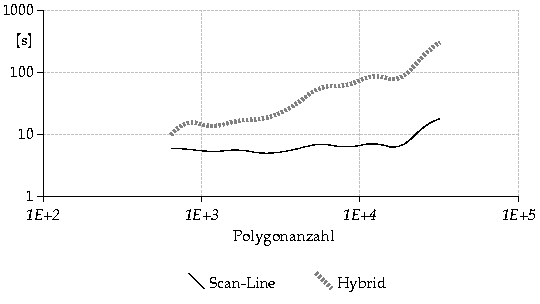
\includegraphics[width=0.44\linewidth]{t-polygon-spline}
\end{tabular}
\caption{Laufzeit - Randknoten-/Polygonanzahl - Diagramm (Spline)}
\label{abb_t_spline}
\diaend


\tabbeg[!ht]
\newcommand*\itema[6]{%
    \emph{#1} & #2 &\small{(~#3~/~#4~/~#5~/~#6)}&}
\newcommand*\itemb[5]{%
    #1 &\small{(#2~/~#3~/~#4~/~#5)} \\ \hline }
\begin{tabular}{|l|rc|rc|}
\hline
\textbf{Tiefe} & \multicolumn{2}{c|}{\textbf{6}} 
    & \multicolumn{2}{c|}{\textbf{7}} \\ \hline
\hline
\itema{Std. Scan-Line }{~5.9}{1.4}{~1.7}{2.8}{0.0}
    \itemb{17.8}{3.8}{~2.2}{~~9.8}{2.0}
\itema{Limited Stack  }{~5.9}{1.5}{~1.6}{2.8}{0.0}
    \itemb{1:15}{3.8}{~3.8}{1:05}{2.0}
\itema{Comb. Scan-Line}{~5.7}{1.5}{~1.3}{2.9}{0.0}
    \itemb{21.5}{3.8}{~5.8}{~~9.9}{2.0}
\hline
\itema{Hybrid         }{56.6}{1.5}{54.0}{1.1}{2.0}
    \itemb{3:49}{3.8}{3:31}{11.7}{2.0}
\itema{Check-Det      }{41.2}{1.5}{37.0}{2.7}{0.0}
    \itemb{3:12}{3.8}{2:58}{~~8.1}{2.0}
\hline
\itema{Debug          }{~7.0}{1.4}{~1.5}{2.1}{2.0}
    \itemb{23.8}{3.6}{~3.6}{14.6}{2.0}
\end{tabular}
\tabend[Laufzeiten unterschiedlicher Algorithmen (\emph{gelenk})]{%
    tbl_diff_verfahren_gelenk}{%
    Laufzeiten [s] unterschiedlicher Algorithmen (\emph{gelenk})}

\dia[!ht]{abb_octstat_algos_gelenk}{%
    Knoten-/Zellenanzahl und Laufzeiten (\emph{gelenk})}{%
    \#Knoten/Normzellen}{nodes-cells-gelenk}{%
    Laufzeiten untersch. Verfahren}{algos-gelenk}

\subsubsection{Auswertung}
Bevor aus den erhobenen Werten Schlussfolgerungen abgeleitet werden k"onnen, 
m"ussen m"ogliche Wertverf"alschungen betrachtet werden:
\begin{description}
\item[Speicherbedarf] Hier ist nicht der reine Speicherbedarf f"ur die 
    Geometrie, sondern f"ur das gesamte Programm cad2octree dargestellt 
    worden. Der zugeteilte Haldenspeicher durch das Betriebssystem kann 
    gr"o"ser sein, als es das Programm ben"otigt. Vom Programm nicht mehr 
    verwendeter Speicher kann erst sp"ater wieder dealloziert werden. 
    Der Speicherbedarf ist zyklisch in Abstand einer Sekunde ermittelt 
    worden. Als Speicherbedarf wird dabei der Maximalwert verwendet.
    F"ur die Me"swerte sind deshalb Abweichungen bis zu 1MB bzw. 10\% 
    einzurechnen. 
\item[Laufzeit] Einerseits werden durch das Betriebssystem und die Hardware 
    Optimierungen wie Caching eingesetzt. Andererseits k"onnen durch 
    unterschiedliche Resourcen-Bereitstellungen des Betriebsystems 
    Abweichungen auftreten, die mit 2 Sekunden bzw. 10\% abzusch"atzen sind. 
\end{description}
Die scheinbar linearen Zusammenh"ange zwischen maximaler Baumtiefe und 
Speicherbedarf und Laufzeit bei 'kleinen' Werten sind deshalb irref"uhrend. 
Aussagekr"aftiger sind Speicherwerte von > 10MB und Zeiten von >10s. 
Ohnehin sind f"ur Aufwandsabsch"atzungen 'gro"se' Werte relevanter.
    
Allgemein ergibt sich eine Korrelation zwischen Speicherbedarf und Laufzeit 
(falls das gleiche Modell bei gleicher Maximalbaumtiefe auf gleicher 
Plattform und das gleiche Generierungsverfahren betrachtet wird).
Die Unterschiede zwischen verbrauchtem Speicher bei unterschiedlichen 
Verfahren sind nur gering.
Im Allgemeinen liefert das Scan-Line-Verfahren die besten Laufzeitergebnisse 
(Die meiste Zeit wird zum F"ullen, beim Hybridverfahren hingegen zur 
Oberfl"achengenerierung ben"otigt).

Betrachtet man die Anzahl der ben"otigten Baum-Knoten, soll lassen sich 
f"ur die hier verwendeten Modelle folgende Erkenntnisse ableiten: 
Die Anzahl der Baumknoten steigt um das maximal Vierfache, falls die 
maximale Baumtiefe um $1$ erh"oht wird. Hingegen verachtfacht sich 
die Anzahl der notwendigen Zellen in einem entsprechenden 
Normzellenaufz"ahlungsschema. Die Zahl der inneren Knoten ist auf maximal 
ca. 20\% der Gesamtknotenanzahl des Oktalbaums beschr"ankt. 
Im Allgemeinen kann durch Kompaktierung die Knotenzahl im Oktalbaum um 
10\% --- 40\% reduziert werden.
Knotenanzahl und Speicherbedarf sind linear voneinander abh"angig 
(n"amlich mit der Konstante Speicherbedarf pro Knoten).

F"ur polygonale Modelle ergibt sich mit der Erh"ohung der Maximalbaumtiefe um 
$1$ maximal eine Vervierfachung der Laufzeit.
Bei Spline-Modellen ist hingegen auch mehr als eine Vervierfachung m"oglich, 
da jetzt die Polygonzahl von der Baumtiefe abh"angig ist (sie vervierfacht 
sich).

%\newpage
%Diagramme t-d\_max fuer untersch. Modelle, fuer untersch. Algorithmen
%Diagramme RAM-d\_max fuer untersch. Modelle, fuer untersch. Algorithmen
%Diagramme t-\#extr. Poly fuer untersch. Algorithmen


%% End of Document


%% End of Document

%% End of Document